\documentclass[12pt,a4paper,utf8x]{article}
\usepackage [frenchb]{babel}
%pour avoir du code source dans le code
\usepackage{listings}
\usepackage{color}
% Pour pouvoir utiliser 
\usepackage{ucs}
\usepackage[utf8x]{inputenc}

\usepackage{url} % Pour avoir de belles url
\usepackage {geometry}

% Pour mettre du code source
\usepackage {listings}
% Pour pouvoir passer en paysage
\usepackage{lscape}
%pour mettre des images
\usepackage{graphicx}


% Pour pouvoir faire plusieurs colonnes
\usepackage {multicol}
% Pour crééer un index
\usepackage{makeidx}
\makeindex

% Pour afficher la bibliographie, mais pas nottoc (Table of Contents), notlof (List of Figures) ni notlot (List of Tables)
\usepackage[notlof, notlot]{tocbibind}


% Pour les entetes de page
% \usepackage{fancyheadings}
%\pagestyle{fancy}
%\renewcommand{\sectionmark}[1]{\markboth{#1}{}} 
%\renewcommand{\subsectionmark}[1]{\markright{#1}} 

% Pour l'interligne de 1.5
\usepackage {setspace}
% Pour les marges de la page
\geometry{a4paper, top=2.5cm, bottom=3.5cm, left=1.5cm, right=1.5cm, marginparwidth=1.2cm}

\parskip=5pt %% distance entre § (paragraphe)
\sloppy %% respecter toujours la marge de droite 

% Pour les pénalités :
\interfootnotelinepenalty=150 %note de bas de page
\widowpenalty=150 %% veuves et orphelines
\clubpenalty=150 

%Pour la longueur de l'indentation des paragraphes
%\setlength{\parindent}{15mm}



%%%% debut macro pour enlever le nom chapitre %%%%
\makeatletter
\def\@makechapterhead#1{%
  \vspace*{50\p@}%
  {\parindent \z@ \raggedright \normalfont
    \interlinepenalty\@M
    \ifnum \c@secnumdepth >\m@ne
        \Huge\bfseries \thechapter\quad
    \fi
    \Huge \bfseries #1\par\nobreaka
    \vskip 40\p@
  }}

\def\@makeschapterhead#1{%
  \vspace*{50\p@}%
  {\parindent \z@ \raggedright
    \normalfont
    \interlinepenalty\@M
    \Huge \bfseries  #1\par\nobreak
    \vskip 40\p@
  }}
\makeatother
%%%% fin macro %%%%

%Couverture 

\title
{
	\normalsize{Master Alma\\
	Université de Nantes\\
	2010-2011}\\
	\vspace{15mm}
	\Huge{Wikitty Publication}\\
	\normalsize{Rapport de stage}
}
\author{FORTUN Manoël\\
	\vspace{45mm}
}

\date{	
	\normalsize{Code Lutin\\
	44, boulevard des Pas Enchantés\\
	44230 Saint-Sébastien-Sur-Loire\\
	\vspace{5mm}	
	Maitre de stage : \emph{POUSSIN Benjamin} \\
	Encadrant de stage : \emph{MOLLY Pascal}
	}
}

%%This is a very basic article template.
%%There is just one section and two subsections.

\begin{document}
\maketitle
\clearpage
\newpage
\null
\newpage

\section*{Remerciements}

Je tiens tout d'abord à remercier Benjamin POUSSIN pour m'avoir permis de faire 
mon stage au sein de Code Lutin, cela aura été une très bonne expérience.

Je voudrais aussi remercier Éric CHATELLIER et sylvain LETELLIER qui m'ont 
aidé tout au long de mon stage.

Je remercie aussi Tony CHEMIT pour ses conseils en terme de bonne pratique et ses
positions généralement intransigeantes justement sur ces bonnes pratiques.

Un merci aussi à Pascal MOLLI pour les cours dispensés cette année,
qui auront été très en phase avec la réalité et ce qui se passe réellement en 
entreprise. Ils ont été parmi les plus réalistes, concrets et utiles parmi ceux
que j'ai eut tout au long de mes formations.

Enfin le remercie l'ensemble des Lutins pour leur accueil chaleureux.

\clearpage
\section*{Résumé}

Ce rapport présente le stage que j'aurais effectué dans le cadre de mon master 2
ALMA, stage effectué chez Code Lutin, une société de service en logiciel libre.
Mon travail aura été articulé autour de Wikitty, une librairie libre 
développée à l'origine par l'entrepise, il s'agit d'un système de base de 
données orienté document, soit clé->valeur. Mon travail aura été autour d'un 
module ce projet, Wikitty Publication dont le concept est de stocker des 
application dans le système de stockage Wikitty, et pouvoir éxécuter l'application
stocker, application qui peut interroger le système de stockage, donc se modifier.
Le but étant d'avoir une application qui peut se modifier comme elle s'éxécute
simplement à travers un navigateur comme pour un wiki. Au départ du stage il 
y avait un prototype simple, fonctionnel, et l'objectif aura été de le 
transformer en un module fonctionnel avec fonctionnalités un peu plus avancées.
Ce concept d'application se base sur le scripting et la possibilité d'interpréter
des langages de script avec d'autre langage, dans notre cas ici du javascript
interprété et éxcuté par du java.\\

Mots clés: Libre, Scripting, Wiki, Wikitty, 





\clearpage
\section*{Introduction}

M2
Rapport qui présente mon stage de fin d'étude.

Concept de wiki

Application en wiki?

Projet libre 
Intéressé pour les bonnes pratiques


\clearpage

\tableofcontents

\section{Code Lutin}

\subsection{Présentation de l'entreprise}


Code Lutin est une Société de Service en Logiciel Libre créée en 2002, elle est
implantée à St Sebastien sur Loire, et travail principalement pour des clients
dans la région du grand ouest.

L'entreprise s'est spécialisée autour des technologies Java JEE et UML:
conception, architectures JEE, outils JEE, MDA (Model Driven Architecture), 
développement/migration d’applications JEE, formation.

L'entreprise étant une SSLL elle travaille uniquement avec des outils issue du
logiciel libre, et autant que celà est possible les projets sur lesquelles elle
va être amené à travailler seront des logiciels libres.

Code Lutin offre les services de : 
\begin{itemize}
\item développement de logiciel (forfait ou régie)
\item l’intégration et de la maintenance de systèmes clés en main
\item support
\item conseil et de la veille technologique
\end{itemize}

Services principalement autour des technologies Java.

%rajuter quelque chose sur le mode de fonctionnement ? A base que ce sont les
%employés qui finalement prennent toutes les déscision. 

\subsection{Acteur du monde libre}

Code Lutin se veut acteur du monde du logiciel libre, l'entreprise soutient des
projets du monde libre. Elle est membre de l'april, une association qui à pour
but de promouvoir et défendre le loficiel libre.

L'entreprise est membre de Alliance libre une association nantaises qui regroupe
les entreprises de la région qui travail pour le libre. Le but étant de
promouvoir le logiciel libre dans l'ouest.

L'entreprise fait aussi partit du réseau libre entreprise qui regroupe des
entreprises françaises proches du logiciel livre, et qui partagent des modes de
fonctionnement similaire et les mêmes valeurs.

% section à étoffer


\subsection{Leurs projets}

En plus de faire du logiciel au forfait et en régie, l'entreprise investit une
grande force dans la recherche et dévellopement, en travail sur leurs librairies
qu'ils utilisent dans leurs divers projet. Mais aussi en travaillant sur des
solutions logiciels qui seront d'abord utilisés en interne, puis proposés
ensuite à des clients une fois que la solution aura été finalisée.

Un exemple, c'est Chorem qui est un outil de gestion d'entreprise pour la
facturation, la gestion des employés, des contrats, etc. Un outil qui à vu le
jour parce Code Lutin ne trouvait pas de logiciel de gestion d'entreprise,
libre.


\clearpage
\section{Organisation du travail}

Pour ce stage au sein de Code Lutin, très vite après avoir pris connaissance 
de mon environnement de travail et des différentes taches qui m'attendait sur
le projet Wikitty Publication, on m'a demandé un planning prévisionnel du travail
(Planning sur la page suivante).

Pour ce stage, et le projet Wikitty Publication, ce qui a été fait, c'est que 
j'ai découpé les spécifications de Wikitty Publication en "grosse" fonctionnalités
de manière à ce que "régulièrement" il puisse y avoir des choses concrètes qui 
fonctionnent.

Les étapes étaient toujours les mêmes dans ces "cycles" de développement:
\begin{itemize}
\item discussion avec mon maître de stage sur les attentes
\item rédaction de spécifications, en détaillant les demandes de sorte à être
le moins ambiguë possible, envoi de ses spécifications sur une liste de 
développement, discussion éventuelle sur ces propositions
\item implémentation des spécifications, avec mise à jour des spécifications 
si nécessaire
\item tests
\item documentation du code
\end{itemize}

De plus toutes les trois semaines au cours de réunions de développement, je 
présentais l'avancé de mon travail et faisais démonstration du fonctionnement
de Wikitty Publication avec les fonctionnalités que j'avais fait depuis la dernière
réunion.

En parallèle, toutes les semaines je faisais un compte rendu par mail sur ce que 
j'avais fais la semaine, ce qui m'avais posé problème et ce que je comptais faire
la semaine suivante. 

D'un point de vue plus technique l'intégralité du projet Wikitty est en JAVA et 
construit avec maven, l'intégration continue est faites par un jenkins. Le projet 
se trouve sur une forge permettant l'assignation de ticket pour les évolutions 
et les corrections de bug. Un sonar est aussi en place pour les métriques et la 
vérification des règles de codage pour le code.

Voici mon planning de travail, il y a des taches qui étaient prévu au départ,
et d'autre qui se sont ajoutées au fur et à mesure. J'aurais assez bien estimé
le temps nécessaire pour certaines taches, certaines m'auront paru plus 
complexe alors qu'elles étaient simples. Mes erreurs d'estimation ont été dut 
à ma non connaissance du domaine au départ, et du fait que je mesurais mal la portée
de certaines fonctionnalités, leurs buts.

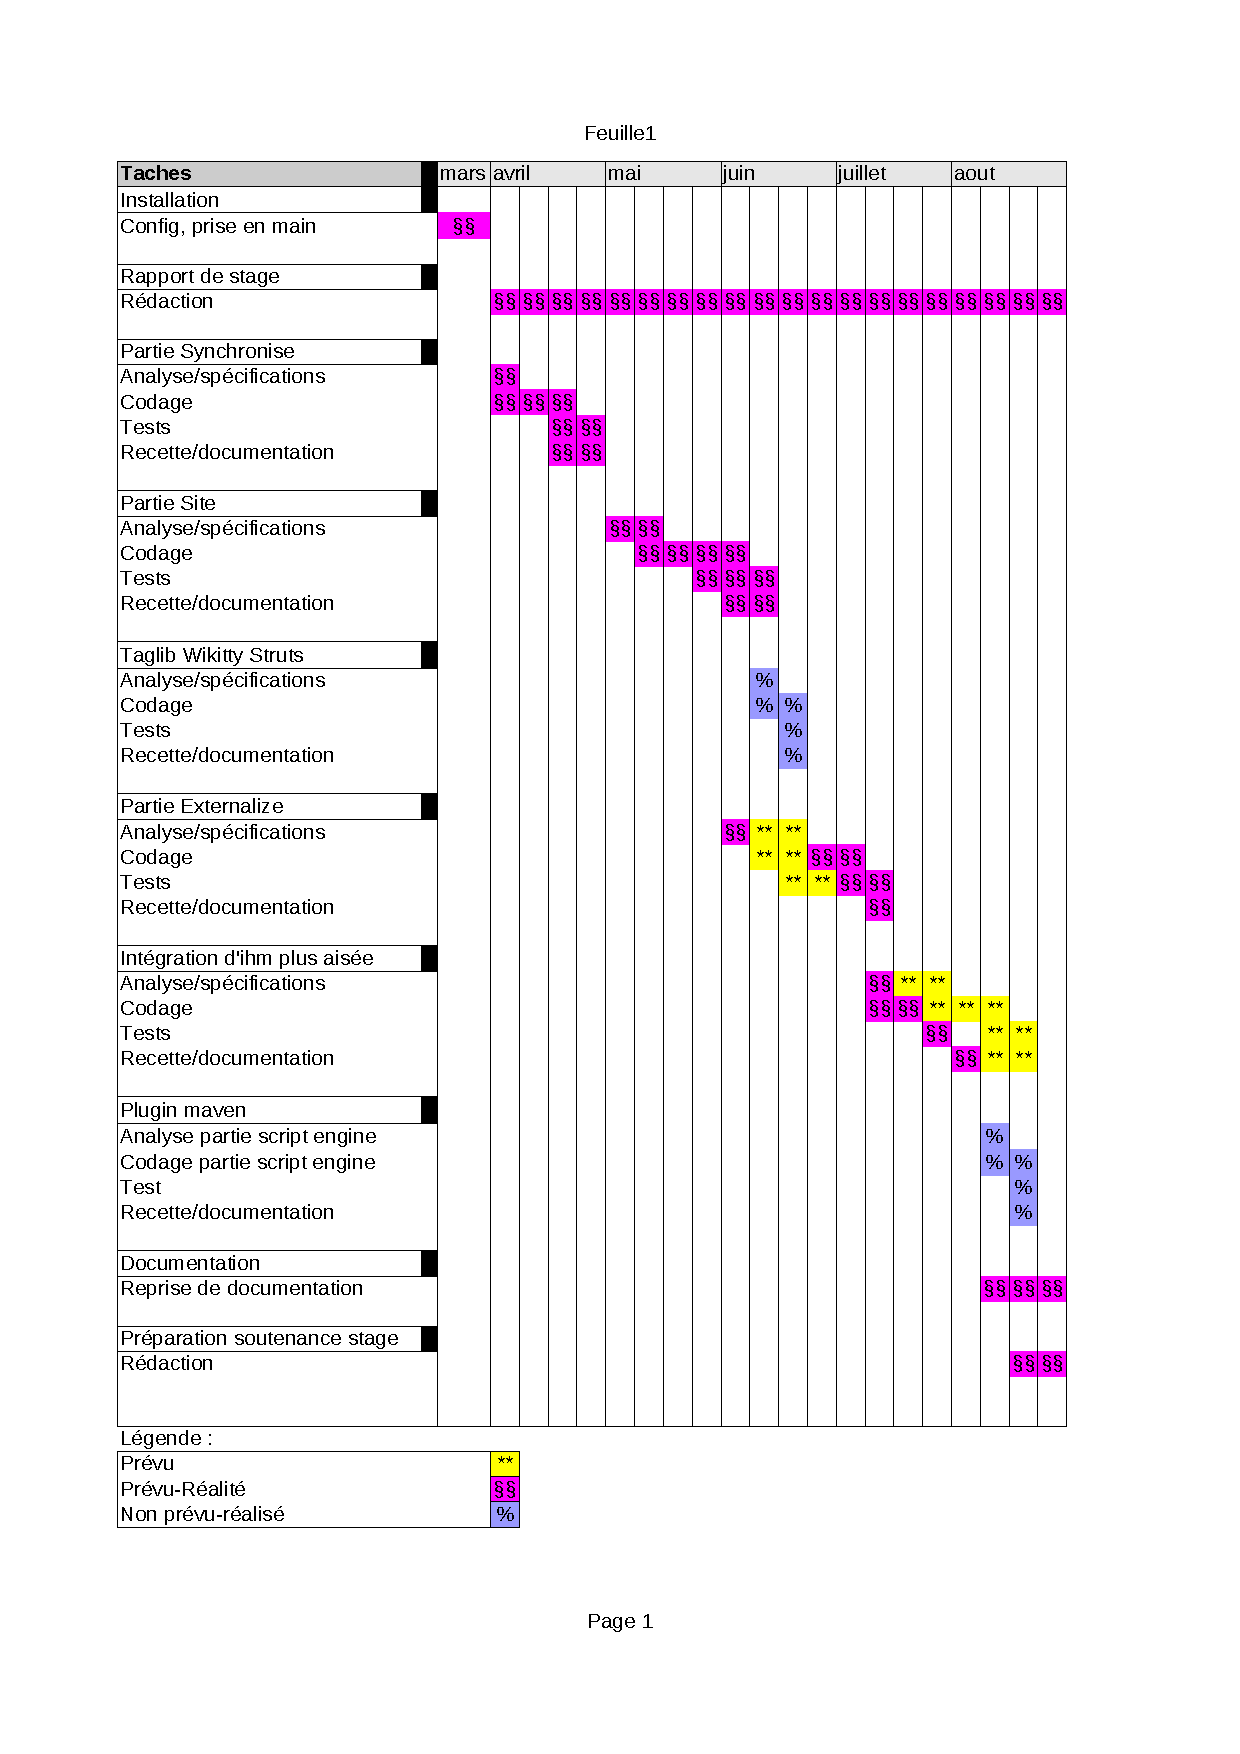
\includepdf{ressources/planningprev2.pdf} 



\clearpage
\section{Projet Wikitty}

Wikitty est un projet important chez code lutin, mon travail à été sur un sous
projet de wikitty, et donc pour le comprendre il est important de présenter
le projet Wikitty.


\subsection{Principe}

Ce projet est une base de données orientée documents et API de persistance pour
Java. Il permet d'enregistrer dans une base clé/valeur des objets wikitty, la
clé est un id généré qui est unique pour chaque wikitty. 

Un wikitty possède des extensions et les extensions possèdent des champs nommés
et chaque champ est une clé à laquelle on associe des valeurs. Et des extensions
peuvent dépendre d'autre extension.

Par exemple une extension personne qui possède deux champs : nom et prénon.
Une autre extension ressource qui possède un champs numéro et qui dépends de
l'extension personne.

Si un wikitty possède l'extension ressource alors ce wikitty possèdera les
champs de l'extension ressource et de l'extension employé, puisque ressource
dépends d'employé.

L'api de wikitty prévois un certain nombre d'extension basique, mais tout
l'intéret est que l'on peut créer ses propres extensions, simplement en écrivant
un modèle uml de classe, qui servira ensuite pour générer les classes java
effectives.

Ensuite il suffit de développer son application simplement en utilisant les
classes générées et les passer à un wikitty service pour le stockage sans plus
se poser de question le tout très simplement.

Cette api à été conçue pour supporter les monter en charge et une utilisation
intensive. Elle supporte aussi la recherche par criteria, et par facette.

La recherche par criteria permet de rechercher des wikitty en fonction de leurs
extensions et des valeurs des différents éléments de ces extensions, sans jamais
écrire de sql, on écrit un critère sur le modèle objet. 

Les facettes permettent de regrouper les résultats de recherche par criteria. 

Tout wikitty posséde un numéro de version, qui évolue en fonction des
modifications faites dessus. L'api prévois que l'on puisse restaurer une version
ciblé d'un wikitty.
%quand wikitty version sera mieux gérer en parler.

\subsection{Existant}

Wikitty sert de base de donnée pour une partie des applications de l'entreprise,
puisque il permet une grande flexibilité. Dès lors ou on peut modéliser les
données en objet on peut les stocker dans avec Wikitty.

Actuellement Wikitty peut être déployé localement, pour une base de données
d'une application, mais il peut être déployé sur un serveur et interrogé grâce
au protocole de communication hessian ou au framework cajo.

Hessian est un protocole de communication pour web service, et cajo est un
framework pour les communications d'application java réparties. 

Une partie des projets actuel de Code Lutin utilise un stockage Wikitty, 
l'objectif est à la généralisation de cette solution pour les projets de 
Code Lutin.

\subsection{Utilisation}

A l'utilisation pour créer ses propres wikitty il faut écrire un diagramme de
classe grâce à l'outil argouml, et que chaque classe porte le stereotype
<<Entity>>, et remplir les différents attribut des classes avec les types
reconnus par java. 

Le fait de stereotyper correctement permet ensuite aux générateurs de générer
les classes java correspondante, et s'assurer qu'elles puissent être stocker
ensuite par Wikitty.

Le déploiement ensuite passe par des fichiers configuration qui permettent la
mise en place des différentes couche de service nécessaire au bon fonctionnement
on peut choisir ainsi d'avoir une base de donnée embarquée ou d'utiliser un
Wikitty service distant.

Celà sans écrire le moindre sql, pour faire des recherches il suffit d'écrire
ses criterias, qui peuvent être construit à partir d'objet wikitty, par exemple 
on veut des wikitty qui ressemble à un modèle, on génère les criterias à partir
de ce modèle.

C'est une approche tout objet, tout java, on se concentre sur l'écriture du code
métier et pas sur l'écriture des couches basses. Puisque le service permet la
sauvegarde, restauration, et recherche.

% Ensuite il suffit d'avoir la base de déployée, et d'utiliser l'interface
% wikittyProxy qui offre les services pour les requêtes de wikitty, les
% sauvegardes, restauration de wikitty. La base de donnée est totalement déléguée
% au wikittyService, pas besoin d'écrire du sql.
% 
% Rajouter que on se sert de wikitty service
% 
% mécanisme de wikitty service et de fichier de propriété liée et tout ça


\subsection{WikittyService, WikittyProxy et WikittyServiceFactory}

Le WikittyService est une interface qui permet de sauvegarder, rechercher,
récupérer des wikitty, il existe des implémentations de service pour différente
base de données, pour des services à distance. Tout les services n'implémentent 
pas toutes les méthodes, par exemple la gestion des authentifications ou la 
gestion d'un cache sont à la charge d'implémentation particulière. Et les
services sont disposés en couche successives pour s'occuper de certain aspect
et déléguant les autres aspect à la couche suuivante.
%ce n'est pas pas un pattern de chain of responsability

%schéma d'encapsulation de wikitty service

La WikittyServiceFactory est une factory au sens pattern, c'est à dire qu'a 
partir de fichier de propriété elle construit et retourne les WikittyServices 
demandé, c'est elle aussi qui organise les couches de service en fonction de ce 
qui est défini dans les fichiers de propriétés.

%exemple de fichier de propriété

Les propriétés ne sont pas directement manipulé, on se sert d'un object 
ApplicationConfig qui permet de gérer différent niveau de propriétés,
avec des propriétés par default si tout n'est pas défini.

Le WikittyProxy est une surcouche qui encapsule un wikitty service et cache 
certaines complexités pour finalement offrir plus de méthodes et des méthodes 
plus simple. Par exemple l'interface WikittyService ne propose que des 
restore de liste de wikitty, alors que le proxy propose des restore de resultat
unique. Dans le cas d'une session ou l'on s'authentifie auprès d'un wikitty 
service, dans ce cas on récupère un jeton, c'est le proxy qui se charge 
d'injecter le jeton dans chaque demande auprès du Service.



\clearpage
parler ici des différentes parties de wikitty publication


\clearpage
\section{Wikitty Publication Synchronisation}

La partie synchronisation de wikitty publication concerne des fonctionnalités
destinées à importer une application auprès d'un wikitty service. Mais pas
seulement, on doit pouvoir synchroniser deux wikittyService quelque soit son
implémentation, que ce soit un client cajo, hessian, un client base de donné ou
même un wikittyService sur file system.

Cette approche de la synchronisation permet une grande flexibilité de
l'application et permet à terme la synchronisation de wikitty entre wikitty
service, et pas seulement ceux concerné par l'aspect publication.

Cette approche implique la création d'une implémentation spécifique d'un wikitty
service pour stocker des wikitty en fichier et restaurer des fichiers en
wikitty.


\subsection{Correspondance Fichiers/Wikitty}

Un fichier est défini par un nom, une extention, un contenu et un chemin.
dans wikitty publication les fichiers sont convertis en fonction de leurs type
en objet wikitty. les fichiers sources sont convertit en WikittyPubText et les
fichiers binaires(eg image, etc) en WikittyPubData.

Ces deux types de wikitty pourrons être dénommé dans la suite sous le nom
WikittyPub. 

Les deux types d'objet ont les mêmes attribut:
\begin{itemize}
\item Name: correspondant au nom du fichier
\item MimeType: crrespondant au type, qui donnera l'extension
\item Content: le contenu binaire pour pour les PubData et textuel pour les
PubText
\item extension: l'extension du fichier original
\end{itemize}

Le mimetype est détermine le contenu, on enregistre en plus l'extension car il
n'y a pas une correspondance parfaite entre extension et mime type, donc pour
ne pas perdre d'information on conserve les deux, par exemple il y a 4
extensions distinct possible pour un mime type: image/jpg. 

A ces objets wikitty on associe un wikittyLabel, c'est un objet qui peut
contenir un ensemble de label différent, un label une chaine de texte.
Par exemple le label : "src.org.chorem.entities" sert ici pour contenir le
chemin menant au fichier sur le file system. Un WikittyPub peut avoir un
plusieurs de label, pour les wikittyPub celà indiquera qu'ils appartiennent à
plusieurs arborescences.

Pour enregistrer un wikitty en fichier, il suffira de construire l'arborescence
des dossiers en fonction du label du WikittyPub. Le nom du fichier sera donné
par l'attribut nom du WikittyPub, son contenu aussi et l'extension aussi, à
défaut d'une extension le mimeType pourra être utilisé pour la déterminer.

Pour assurer la restauration d'un WikittyPub qui aura été sauvegardé en fichier,
il faut enregistrer en plus des informations supplémentaire. Comme tout Wikitty,
les WikittyPub possèdent un numéro de version ainsi qu'un id qui les identifient
de façon unique.

Il faut donc enregistrer ses informations, de plus il faut que le wikitty
service sur file système gère les modifications sur Wikitty et donc modifie la
version des Wikitty si besoin.

La solution qui à été trouvée pour celà est les fichiers de propriété dans un
dossier ``.wp/''. 

On distinguera deux fichiers de propriétés pour les informations un qui 
conservera les id des wikitty lié à leur nom de fichier. Et un autre fichiers de
propriété qui conservera un checksum, la version et les id aussi. En sus de
la sauvegarde des ``meta information" des Wikitty, ce fichier de propriété
conservera le nom du label courant, rendant immediat la restauration (pas
besoin de traitement complexe sur les noms de fichier/dossier).

On conserve les id dans un premier fichier puisque celà permet simplement de 
récupérer l'ensemble des id et leurs noms de fichier lié sans avoir besoin de 
faire le tri parmis toutes les propriétés enregistrées. On converse l'id aussi 
dans un autre fichier de propriété, à défaut d'avoir un system d'enregistrement
clé/valeur bidirectionnel. 

La propriété checksum sera utilisée pour enregistrer la somme de controle de 
l'objet lors de son enregistrement, pour plus tard, savoir si celui ci à été
modifié depuis lors.

Exemple pour un contenu de file system:
\begin{verbatim}
 +racine
 |script.js
 |scripttut.js
 |image.png
 |+.wp
 ||id.properties 
 ||meta.properties 
 |+directory2
 ||script3.js
 ||+.wp
 |||meta.properties
 |||id.properties 
 ||+directory3
 |||truc.js
 |||+.wp
 ||||meta.properties
 ||||id.properties 
 |+directory22
 ||machin.png
 ||+.wp
 |||versions.properties
 |||id.properties 
\end{verbatim}


Exemples de fichiers de propriétés:
\begin{verbatim}
racine/.wp/meta.properties:

current.label=racine
script.js.version=numéroVersion7
version.scripttut.js=numéroVersion
version.image.png=numéroVersion
checksum.script.js= checksum
checksum.scripttut.js= checksum
checksum.image.png= checksum
id.image.png=uubdazudba
id.scripttut.js=11daz5facz
id.script.js=jbdub1dza8
\end{verbatim}

\begin{verbatim}
racine/.wp/id.properties:

uubdazudba=image.png
11daz5facz=scripttut.js
jbdub1dza8=script.js
\end{verbatim}

\subsection{Un wikitty service file system}

Un wikitty service implémenter pour système de fichier doit pouvoir enregistrer
des wikitty en fichier et inversement. Pour se faire il se servira des fichiers
de propriété précédement exposé, et des conversions telles qu'elles le sont
proposées.

En plus de la sauvegarde, restauration et supression, ce type de wikitty service
doit, c'est la base du système de synchronisation, gérer les recherches par
critère des wikitty comme si il était stocké de façon classique dans une base.

Pour correctement gérer ces options de sauvegarde, restauration, gestion de
version des wikitty, pour tout appel à la recherche ce wikitty service indexe
l'ensemble des fichiers:
\begin{itemize}
\item vérifie si il y a des nouveaux fichiers en comparant les valeurs dans les
fichier de propriétés ``id.properties''. Si il ya des nouveaux fichiers il créé
des id, calcul les sommes de contrôle et enregistre le tout dans les fichiers de
propriétés.
\item il vérifie la somme de controle des fichiers existant, et incrémente la
version pour ceux qui ont changé, et il met à jour la somme de contrôle
\item il cherche si des fichiers ont été supprimé, et le cas échéant enlève les
infos concernant le wikitty correspondant au fichier
\end{itemize}

Avec ces fonctions le wikitty service file system est ``complet'' pour la
synchronisation.

Le mécanisme qui indexe créer automatiquement les fichiers de propriété
nécessaire, ce qui implique que une arborescence de fichier peut être converti
en wikitty de cette façon, nul besoin d'initialiser un espace de travail en en
le créant à partir de wikitty, tout dossier peut devenir ``une base wikitty''.

\subsection{Fonctionnalitées de synchronisation}

\subsubsection{Sync}

La fonctionnalité sync permet de transférer l'ensemble des wikittys ciblés par 
l'uri, d'un service wikitty à un autre. Son fonctionnement doit est similaire à
la commande linux "rsync".

Quelques options on été reprise:
\begin{itemize}
\item Recursion pour savoir si l'on s'occupe des sous labels du label ciblé.
\item Update, qui permettra de mettre à jour ce qui est présent et antérieur
sur la cible et d'y envoyer les nouveaux wikitty. Par défaut cette option est
active, et sera desactivée lorsque les autres options (delete ou existing)
seront choisis.
\item Existing qui est un update mais sans l'envois des nouveaux fichiers, on
envois juste ce qui à été mis à jour et qui existe sur le wikitty service cible.
\item Delete pour supprimer dans le wikitty service cible, ce qui n'existe plus
dans le wikitty service origine.
\end{itemize}

La suppression n'est pas une vraie suppression elle se contente de supprimer le 
label ciblé du wikitty, l'éventuel suppresion définitive du wikitty si celui ci
se retrouve sans label est à la charge du service.

Le type de l'implémentation des wikitty service nécessaire pour la communication
avec les uris passé en paramètre sont à la charge d'une factory. 

La commande:

''wp sync [--norecursion] [--delete|--existing] [URI orgirine] [URI cible]''

Avec URI sous forme: 
\begin{itemize}
\item file:///truc/machin/\#label
\item hessian://www.adresse.com:8827/etc/etc\#label
\item cajo://www.adresse.com:8827/etc/etc\#label
\end{itemize}

Evidement le path et le label pour une uri de type file détermine l'espace de
travail wikitty. eg: /truc/machin/label est le repertoire racine

Les labels de l'uri cible et origine peuvent être différent, ce qui signifie que
les labels ne sont pas forcément transmit, le wikitty sur la cible est modifié
mais pas ses labels.

Dans le cas de wikitty qui n'existe pas dans la cible, on remplacera le label
origine qui à permis de trouver ces wikitties par le label cible.

\subsubsection{Commit/update}

Les fonctionnalités commit/update sont des alias pour la commande sync.
L'utilisation de ces commandes implique la présence d'un espace de travail
précédement initialisé avec la commande sync.

Les commandes commit et update permette de ne pas avoir besoin de préciser le
wikitty service cible de la synchronisation, synchroniser avec le dernier
wikitty service utilisé pour. Celà implique que un wikitty service file system
enregistre l'adresse du wikitty service avec lequel on le synchronise.

Pour ce faire un fichier de propriété enregistre l'adresse du wikitty service
servant pour une synchronisation.

Un commit sera équivalent à un sync de l'espace de travail local vers un autre
wikitty service. 

Un update sera équivalent à un sync d'un autre wikitty service vers l'espace de
travail local.

La commande:

''wp [update|commit] [--norecursion] [--delete|--existing] [label] [URI file]''

L'URI file est optionnelle, si pas précisée on va commit/update le dossier 
courrant.

Pour le commit/update, on doit forcément préciser le label pour le wikitty 
service cible, celà pour permettre de commit ou update au bon endroit.
La commande supporte évidement les mêmes options que pour une commande sync, en
toute logique.


\subsection{Fonctionnement de sync}


Une synchronisation entre deux wikitty service se fait en comparant les wikitty
qu'ils ont chacun, wikitty qui possèdent soit des labels préçis ou des labels
commençant par une chaine, fonction de l'option récusion.

On distinguera les wikittys qui existent dans les deux services, ceux présent
uniquement dans le wikitty service cible et ceux uniquement sur le wikitty
service d'origine.

Ensuite en fonction de l'option de synchronisation ces différentes collection de
wikitty sont utilisé.

Dans le cas d'une uptate tout les wikitty qui existe uniquement dans l'origine
son envoyé, et ceux présent dans les deux sont mis à jour.

Dans le cas d'un existing seulement ceux présent dans les deux sont mis à jour.
Et dans le cas d'un delete on va supprimer les labels des wikitty seulement
présent sur la cible.


\clearpage
\section{Wikitty Publication Site}

La partie site de Wikitty Publication concerne des fonctionnalités
destinées à l'administration et les éléments coeur du moteur de publication
comme l'interprétation du code contenu dans les WikittyPubText. 

Ces fonctionnalités principales sont :
\begin{itemize}
\item Raw, qui permet l'affichage des WikittyPubData exemple des images
\item Edit, qui permet de créer ou d'éditer des Wikitty
\item Eval, qui permet l'évaluation du code contenu dans un WikittyPubText
\item View, qui permet l'affichage et la recherche des Wikitty
\end{itemize}

Un premier prototype avait été réalisé c'était la base de travail, ce prototype
était fait avec des jsp/servlet simplement sans support d'un quelconque
framework comme struts.

Le travail sur cette partie de publication se concentrait donc sur
l'amélioration de ce prototype sous différent aspect.


\subsection{Migration vers struts}

Le premier aspect de l'amélioration du prototype était de migrer les jsp/servlet
vers le framework struts. Struts est un donc un framework qui permet un bon
support du modèle MVC pour les applications web.

Struts permet au dévelloppeurs de se concentrer sur la vue et le modèle de son
application Web, à la charge de struts l'aspect contrôleur du modèle MVC. En
effet on peut définir l'enchainement des actions effectuées et la page qui sera
affiché en conséquence.

Dans struts on parle d'action, de package et d'intercepteur, les packages
regroupent les actions et les piles d'intercepteurs, ces packages peuvent en
étendre d'autre et donc hériter de leurs propriétés. Les packages peuvent
posséder un 'namespace' qui leur permet d'être défini pour un sous espace de
l'application.

\begin{figure}[!ht]
\centering
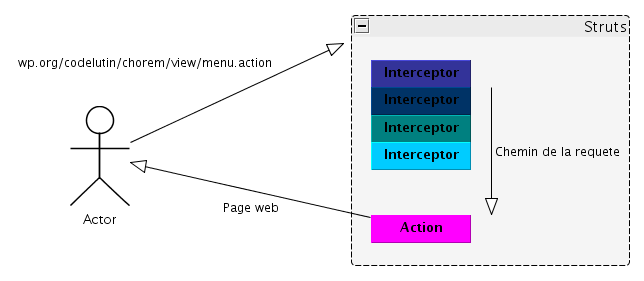
\includegraphics[height=6cm,width=17cm]{image/strutsexplain.png}
  		\caption{Diagramme Struts}
  		\label{diagstruts}
\end{figure}

Les intercepteurs et piles d'intercepteur sont des objets qui effectue un pré
traitement sur les requêtes http reçu par l'application, la figure \ref{diagstruts}
montre le cheminement possible d'une requête. Le champ d'action des intercepteurs
est grand, ils ont accès à la session, le contexte etc.

Les actions permettent de décrire l'enchainement des 'écrans', les classes java
qui doivent éxécuter un traitement après la validation d'un formulaire jsp, la
jsp à afficher et d'autres.

Cette configuration de struts se fait grâce à des xml, ensuite il suffit
simplement d'écrire des classes java qui implémentent des interfaces
spécifiques. Je dévelloperais pas plus le fonctionnement de struts.

Un des aspect important de la migration vers struts aura été la conversation des
url correspondant aux actions de publications, les url doivent être sous cette
forme : 
\begin{verbatim}
/[contextData]/[contextApps]/[action]/[mandatory_args]?[args key=value]
\end{verbatim}

Les actions: 
\begin{itemize}
\item Raw
\item Edit
\item Eval
\item View
\end{itemize}

Le context sert pour trouver le bon Wikitty Service. Les mandatory args servent
pour les actions: Raw, Eval et Edit pour trouver le bon objet wikitty
correspondant. Par exemple :

\begin{verbatim}
/edit/elt_id:928b573e-b76f-4ffc-95a1-205798034330 
/eval/WikittyPubText.name:Wiki
/raw/Wiki
\end{verbatim}

%format des urls à mettre ici

Respectivement :
\begin{itemize}
\item l'action edit pour le wikitty avec l'id correspondant
\item l'action eval pour le wikittyPubText qui possèdent le champ name égal à
Wiki
\item l'action raw pour le wikitty qui possède un champ nom égal à Wiki
\end{itemize}

Ces deux derniers exemples montrent plusieurs formats pour retrouver un même
wikitty. 

Les actions de publication Raw et Eval sont un peu particulières, contrairement
aux deux autres elles n'ont pas de page jsp de rendu, les actions View et Edit
ont des jsp pour l'affichage et l'édition/création de wikitty.

L'action Raw par exemple pour les WikittyPubText et PubData affiche le contenu
des wikitty en fonction de leur mime type, et donc construit lui même son rendu
html sans passer par une jsp.

L'action Eval elle sert sert du mime type d'un WikittyPubText pour déterminer le
langage associé au contenu et finalement execute le code, le resultat de
l'éxécution est donc ensuite renvoyé en tant que résultat.

\subsection{Moteur d'évaluation}

Le moteur d'évaluation s'appuie sur le concept de scripting comme précédement 
évoqué, on a pu voir que dans les adresses des actions il ya deux paramètres
dont je n'ai pas vraiment parlé: \emph{contextData} et \emph{contextApps}.

C'est qu'ils prennent toutes leurs importance dans le méchanisme d'évaluation,
ce méchanisme est délégué au script engine qui va intépréter le contenu
d'un wikittyPubText en fonction de son mimeType et renvoyer simplement un 
wikittyPubData de la même façon.

Dans ce cadre contextData sert pour savoir connaitre les propriétés, donc
quels wikitty service instancier. Comme précédement expliqué les wikitty service 
sont instancié avec des fichiers de propriété, par défaut il existe deux fichier
dans l'application qui définisse un wikitty service "classique" avec une base
de données h2, un dossier de stockage, ainsi qu'un wikitty service sur jar
en fallback. 

Le contextData sert pour deux choses dans ce cadre, il permet de charger un 
fichier de propriété supplémentaire s'il existe voir sur la figure 
\ref{propertiescontext} , et de définir le dossier de stockage de la base. 

\begin{figure}[!ht]
\centering
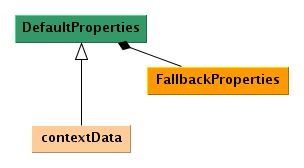
\includegraphics[height=3cm,width=6cm]{image/propertiescontext.png}
  		\caption{Fonctionnement du ContextData}
  		\label{propertiescontext}
\end{figure}

Si par exemple l'adresse de l'action est \verb!/codelutin/chorem/eval/menu.action!
alors on chargera les propriétés par défaut, on cherchera un fichier de propriété
codelutin s'il existe(qui peut écraser des propriétés existantes) et un sous dossier
sera créé pour le contexte de l'application \verb!codelutin!, isolant totalement
d'un autre contexte \verb!/wp/chorem/eval/menu.action! par exemple, ça ne sera
pas les mêmes base de donnée, on peut isoler ainsi les contextes

ContextData sert donc pour isoler les services et leurs bases.

ContextApps lui son rôle est "d'isoler" les applications et éviter les collisions
de nom entre les wikitty, les noms ne sont pas unique et on peut se retrouver
dans un même wikitty service avoir plusieurs wikittyPub qui ont les mêmes nom par
exemple: "menu". Le but est d'éviter des confusions, par exemple une action
\verb!/codelutin/chorem/eval/menu.action! on va aller chercher le wikittyPub 
avec le nom "menu" dont l'un des labels commence par "chorem", celà permet de 
regrouper les applications sous les mêmes label, ainsi si dans le contenu du 
"menu" il y a un appel vers un autre wikitty le moteur "sait" qu'il doit 
aller le chercher sous le même label.


\subsection{Ajout d'un mécanisme de login/logout}

Les couches sécurité des wikitty service s'occupe déjà d'un mécanisme de login
et d'une gestion des droits en fonction. Les utilisateurs sont stocker en tant
que wikitty dans la base et on peut attribué des droits à ces utilisateurs.
Ensuite via un wikitty service on peut se loger, sur une authentification on
récupére un jeton qui sera à passer pour chaque action, celà est géré par le
wikitty proxy qui encapsule le wikitty service.

Donc pour vérifier qu'une authentification s'est bien passé il faut regarder
dans le proxy si l'utilisateur est présent. Dans le cas de wikitty publication
au moment de l'action de login, délégué au proxy, on va stocker le jeton et
l'utilisateur dans la session.

Evidement le mécanisme de Logout lui nettoie simplement la session en la vidant
de ces informations.

Ensuite le fonction de la gestion de l'authentification se repose sur le
méchanisme d'intercepteur et de package de struts. On défini une pile
d'intercepteur personalisé qui en plus de la pile par defaut rajoute un
intercepteur d'authenfication qui vérifiera la présence des informations
utilisateur dans la session, et bloquera l'accès à la page demandé si
l'utilisateur n'est pas authentifié.

On définit que l'accès aux actions publication utilise cette pile d'intercepteur
qui gère l'authentification, c'est ainsi que fonctionne le méchanisme dans
wikitty publication.

\subsection{Amélioration des pages d'affichage et d'édition}

Les pages d'édition et d'affichage des wikitty étaient relativement simple, le
but étant une administration simple et efficace des wikitty. L'amélioration de
ces pages à consister en la correction des bugs présent déjà dans le prototype.

Par exemple le support pour les recherches dans wikitty dans la page view,
dans le prototype cette recherche était très limité et donc ne fonctionnait pas
très bien. De plus l'affichage des résultats nécessitait une amélioration.

Ensuite pour l'interface d'édition des wikitty j'ai intégré un décorateur de
Text Area qui permet une colorisation du contenu du champ, on peut choisir le
langage présent dans le champ pour avoir une colorisation, de l'indentation, des
outils de recherche/remplacer et d'autre, basiquement une sorte d'ide pour
faciliter le dévellopement de code dans les WikittyPubText.

% mettre screen shot du décorateur de textarea


\subsection{Mécanisme de multicontext}

Cette fonctionnalité consiste en fait à l'encapsulation par un wikitty service
de deux autres wikitty service, quelque soit leurs natures, c'est un 
WikittyFallbackService. On peut voir un schéma de fonctionnement sur la figure
\ref{diagmulticontext}

Ce multi contexte éxécute ses recherches un wikitty service principal, et
compléte ses recherches si besoin avec les données du wikitty service dit
fallback. A titre d'exemple si on effectue une recherche que l'on réclame un
résultat d'au moins 30 wikitty, si à l'issue de la recherche sur le wikitty 
service principal il n'y a pas 30 wikitty, alors on cherchera sur le service
fallback pour compléter la recherche. 

Ainsi si l'on cherche à retrouver un wikitty particulier avec son id, si il
se trouve sur le principal ça sera le wikitty du principal qui sera renvoyé, 
par contre si il ne se trouve pas sur celui si, on ira le chercher sur le second
service.

De même l'écriture s'effectue sur le service principale, on n'écrit pas sur le
service de fallback.

\begin{figure}[!ht]
  	%[height=12cm,width=15cm]
\centering
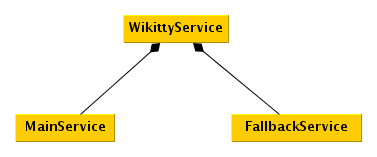
\includegraphics{image/multicontext.png}
  		\caption{Diagramme multicontexte}
  		\label{diagmulticontext}
\end{figure}


Son utilisation n'est pas nécessairement limité à Wikitty Publication, il s'agit
finalement d'une implémentation différente de l'interface wikitty service. 

Ce mécanisme peut permettre la surcharge d'un wikitty, dans le sens ou on peut
modifier un wikitty qui aura été chargé depuis le fallback, mais à la sauvegarde
il sera restaurer depuis le wikitty principal, puisque celui ci est prioritaire.

On peut avoir ainsi un wikitty service statique, et un autre dynamique, par
exemple le wikitty service statique qui serait partagé et utilisé par d'autre
wikitty service multicontext, une base commune de wikitty. 

Ce Wikitty Service à été pensé et écrit pendant l'enrichissement de la partie 
site de Wikitty Publication, l'idée d'utilisation d'un tel service, est la 
mutualisation d'une application dans un wikitty service, et que cette 
application utilise des données issue de d'autre service. On mutualise le code 
métier, de sorte que plusieurs clients puissent utiliser la même application, 
avec le même service, mais que leurs données soit sur leurs services, 
le service fallback contiendrait l'application et le service principal 
l'application.

\subsection{Intégration d'interface graphique}

Les applications éxécuté au sein de wikitty publication le seront à travers 
un navigateur web donc le résultat présenté dans un format compatible.
Donc générélament pour proposer des choix utilisateurs il faudra des interfaces
en html.

Le html peut être aisément intégré dans du javascript et quand l'évaluateur
evaluera le javacript et écrira le html contenu dans les variables javascript
mais cette solution rends l'écriture du code interface pénible.

La solution la plus simple qui a été trouvé est d'avoir la possibilité d'écrire 
du html (pour le moment plus tard d'autre langage) et de faire comme si on était
dans une jsp, quand on a besoin d'écrire code on ouvre des balises : \verb!<% \%>!
ou \verb!<%= \%>! et on écrit le code correspondant.

Ce qui se passe derrière c'est que on inverse le code, ce qui se trouve entre
les balises devient du code exécutable, et ce qui se trouve autour se retrouve
décoré. Tout simplement comme si initialement le html avait été intégré dans
le code d'un langage interprété par publication.

Une autre solution était envisagé, qui voulait considérer le html comme un langage
supporté par publication, et extraire les éléments de binding mais c'était plus 
compliqué.

Une nouvelle fois on va jouer avec le mimeType pour les WikittyPubText qui 
seront des IHM, on leur mettra un mimeType composé de forme: text/html.javascript,
ce qui signifiera que l'on a un WikittyPubText qui entre les balises de délimitation
contient du javascript, et que l'on doit se servir des rêgles de décoration javascript.
Et que après décoration le contenu sera de mimeType: text/javascript.

Voir annexes pour exemples de décoration interface.

\clearpage
\section{Wikitty Struts}

Cette partie sur Wikitty n'était pas prévu au départ, mais à l'utilisation
il s'est avéré que le développement d'un tel module était nécessaire, et que
le travail précédemment effectué sur la partie site de Wikitty Publication
pouvait rendre la tache plus rapide.


\subsection{Objectfifs}

L'édition de wikitty ou tout simplement l'utilisation de wikitty au sein de 
formulaire deviennent des éléments récurents dans les applications développées 
chez code lutin. Cela puisque devient Wikitty une solution plus utilisée pour 
le stockage.

L'objectif de ce module wikitty-struts a donc été de créer une taglib permettant
une génération des formulaires pour les wikitty, afin de ne pas avoir à refaire
ce que l'on a déjà fait pour une autre application.

Pour avoir une tag lib la plus complète possible, il a été décidé d'en faire une
qui marcherait de la même façon que la taglib struts de base, et se resservirait
de ses mécanismes interne, avec les templates.

\subsection{La création d'un tag}

\begin{figure}[!ht]
  	%[height=12cm,width=15cm]
\centering
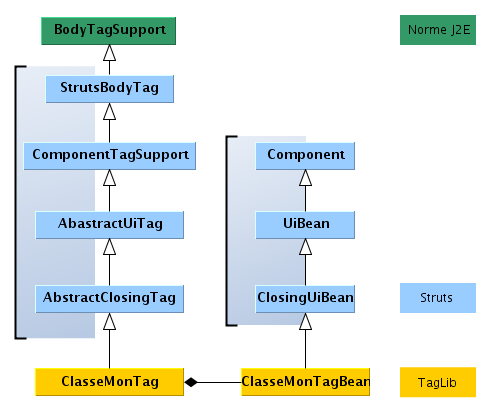
\includegraphics[height=7cm,width=9cm]{image/explicationTag.png}
  		\caption{Diagramme des tags avec struts}
  		\label{diagtagstruts}
\end{figure}

La création d'un tag classique, sans struts se fait par héritage de classe 
tel que "TagSupport" qui est une des classes définie dans la norme J2E pour la 
création des tags. En plus de la définition de la classe java, il faut écrire
dans un fichier xml (.tld) la définition du tag. La création de tag ainsi oblige
à écrire le code html directement dans le corps de la classe ou de devoir prévoir
l'architecture de support pour des templates.

Les templates permettent en fait de séparer le rendu du post-traitement effectué
sur les attributs d'un tag, il permettent aussi de supporter plusieurs "thèmes", 
c'est à dire des collections de css pour changer le rendu, etc.

Faire des tag comme struts c'est un peu différent donc, sur la figure \ref{diagtagstruts} 
on voit qu'il y a une certaine architecture déjà mise en place. Il y a une chaine 
d'héritage étendant la norme pour les tag, et de l'autre une chaine d'héritage 
de classe spécifique à struts. 

Pour créer des tags spécifiques on se place en bout de chaine, comme on le voit 
avec \emph{classeMontag} en héritant de \emph{AbstractClosingTag} on ne fait pas
grand chose, on délègue à la classe héritant de \emph{ClosingUiBean} qui contient 
elle la logique de traitement des éléments du tag. Ensuite il faut définir le
template écrit en \emph{freemarker}, qui lui contient le code html effectif 
qui sera écrit avec les éléments récupérés par la classe héritant de \emph{ClosingUiBean}.
Il faut aussi écrire le fichier tld pour la description.\\
\\
Pour résumer la création d'une taglib c'est:

\begin{itemize}
\item un fichier descripteur pour la taglib avec chaque tag de décrit 
\item une classe héritant de ClosingUiBean pour chaque tag
\item une classe héritant de AbstractClosingTag pour chaque tag qui délègue à son ClosingUiBean correspondant
\item des fichiers de template en freemarker pour chaque tag
\end{itemize}

Exemple de template freemarker:

\lstset{ %
language=HTML,                % the language of the code
basicstyle=\footnotesize,       % the size of the fonts that are used for the code               % where to put the line-numbers
  % the size of the fonts that are used for the line-numbers
                  % the step between two line-numbers. If it's 1, each line 
keywordstyle=\color[rgb]{0,0,1},
                      % will be numbered
numbersep=5pt,                  % how far the line-numbers are from the code
showspaces=false,               % show spaces adding particular underscores
showstringspaces=false,         % underline spaces within strings
showtabs=false,                 % show tabs within strings adding particular underscores
tabsize=2,                      % sets default tabsize to 2 spaces
captionpos=b,                   % sets the caption-position to bottom
breaklines=true,                % sets automatic line breaking
breakatwhitespace=false,        % sets if automatic breaks should only happen at whitespace
title=\lstname,                 % show the filename of files included with \lstinputlisting;
                                % also try caption instead of title
escapeinside={\%*}{*)},         % if you want to add a comment with
morekeywords={project,modelVersion,groupId,description,build, plugin,plugins,configuration, applicationName, wikittyServiceUrl, artifactId,serverID,uploadUrl} 
}



\begin{lstlisting}
<#include "/${parameters.templateDir}/${parameters.theme}/ws-label-commons.ftl" />
<select 
<#include "/${parameters.templateDir}/${parameters.theme}/ws-commons.ftl" />
 size="${parameters.selectSize}">
<#assign optionKeys = parameters.value/>
    <#list optionKeys as optionKey>
	<option value="${optionKey.valeur}"
	<#if  optionKey.valeur==parameters.value >
		selected
	</#if>
	> ${optionKey.description} </option>
	</#list>
</select>
\end{lstlisting}

Ce template, est le template pour le rendu en combobox ou liste de sélection,
il y a les éléments html et les éléments de langages freemarker. Avant que le
template soit remplit, les classes java correspondantes au tag remplissent 
un map de paramètres à laquelle a accès le template, d'où les structures de contrôle
pour itérer dans cette exemple. 


\subsection{La taglib wikitty struts "ws"}

Les tags ainsi développés ont deux utilisations possibles, la création d'un 
formulaire d'édition de wikitty, ou la création de formulaire utilisant les 
champs de wikitty comme champs. 

La différenciation de l'utilisation des tags passent par l'utilisation du tag 
de la taglib ws:form, qui implique que dans ce cas on se trouve dans l'édition d'un
wikitty.

A l'utilisation si on met seulement le tag \emph{ws:form} et la source de donnée 
(le wikitty) un formulaire basique va être créé en fonction du type des champs
du wikitty. Ensuite en utilisant les autres tag ou différents attributs du tag 
\emph{ws:form} il est possible de choisir d'exclure de l'édition des extensions,
des champs ou de choisir le type d'affichage pour un champ donné (et identifié
par son nom complet soit nomExtention.nomChamp).

En plus de fournir des tags pour la création de formulaire, la tag lib propose 
une action qui permet de prendre en compte les modifications de wikitty envoyées
par le formulaire. Il s'agit d'une action abstraite struts que l'utilisateur à 
besoin d'étendre pour implémenter la méthode accédant au proxy.

Tag commun aux deux types d'utilisation:
\begin{itemize}
\item ws:hidden permet d'insérer le champ en tant que champs caché
\item ws:boolean permet d'insérer le champ en tant que checkbox 
\item ws:textArea permet d'insérer le champ en tant que textArea
\item ws:textField permet d'insérer le champ en tant que textField
\item ws:date permet d'avoir un composant intelligent pour les dates 
\item ws:selectFixed permet d'afficher un combobox avec des valeurs fixées à 
l'avance, sera sélectionnée celle correspondant au champs wikitty liés
\item ws:selectCriteria permet d'afficher un combox box avec des wikitty, 
sera sélectionnée le wikitty correspondant à l'id du wikitty du champ
(utilisé donc dans le cadre de relation entre wikitty)\\
\end{itemize}

Tag spécifique pour la création de formulaire:
\begin{itemize}
\item ws:form tag pour la création d'un formulaire d'édition des wikitty \\
\end{itemize}

Tag spécifiques à l'utilisation champ:
\begin{itemize}
\item ws:selectAssociation tag pour l'affichage de champ wikitty de type collection
\item ws:select tag pour l'affichage de collection de wikitty en tant que list ou combobox html
\end{itemize}




\clearpage
\section{Wikitty Publication Externalize}

La partie externalize de wikitty publication concerne les fonctionnalités 
d'externalisation des wikitty. C'est à dire prendre des wikitty stocker sur un 
système de fichier, via le service correspondant précédement dévellopé, compiler
ces wikitty et les stockers dans un jar.

L'objectif recherché par cette partie de wikitty publication est la performance,
en ayant du code compilé on gagne évidement en rapidité d'éxécution des wikitty
compilé. Et du code non modifiable, par exemple dans le cadre de l'utilisation 
multicontexte, on pourrait avoir un service s'appuyant sur des wikitty stocké 
dans un jar.

Comme pour la synchronisation vers file system, sont concernés par ce méchanisme
uniquement les Wikitty représentable sur file system, comme les wikittyPubData,
qui ne seront pas affecté par le méchanisme, et les wikittyPubText qui eux seront
compilé dans le processus d'externalisation.

Un des objectifs, plus secondaire, est la possibilité d'intégrer ce méchanisme
en tache Ant, ou un plug in maven.

\subsection{Une nouvelle extension de wikittyPub}

Les wikittyPubText qui auront été externalizé, et donc compilé, doivent toujours 
être considéré comme des wikitty, avec toutes les propriétés liées. Pour ce 
faire on défini une extension de wikittyPubText qui contiendra un champ nommé 
ByteCode de type tableau de byte.

Ainsi pour ce type de wikitty d'un coté on aura le code original du 
wikittyPubText dans le champ content et le code java compilé dans le champ
ByteCode. Celà permet d'avoir l'original dans le cas où l'on voudrait écrire
un nouveau wikitty avec le même code, ou dans le cas d'une surcharge si 
multicontexte.

\subsection{Mechanisme de transformation/compilation}

Tout le méchanisme de transformation des wikittyPubText en wikittyPubTextCompiled
doit doit respecter la finalité de ces wikitty, c'est à dire que le code qu'ils
contiennent soit exécutable et exécuté. 

Quelque soit le contenu des wikittyPubText ils sont compilé, normalement pour les
langages visé, tel le javascript on ne peut pas le compilé comme on le pourrais 
pour du java. Ce qui est fait c'est que ce code est encapsuler dans un morceau
de java qui invoque le script engine chargé de son exécution. 

Pour les langages comme le java on met simplement le code dans une méthode qui 
sera appellée quand on évaluera le code.

Pour ces deux cas le code java qui décore est presque le même, on à une classe
abstraite de décoration qui possède une méthode abstraitre eval, qui prend en 
paramètre la map contenant les Bindings[ref binding] nécessaire à l'éxécution 
du code.

% code décorer java
% code décoré non java TODO

En dehors de la compilation et décoration des wikitty, le mechanisme est 
relativement simple. On sélectionne tous les wikitty du dossier local où on
se trouve avec le service file system, on créer un dossier temporaire, 
on y écrit les wikitty, on compile ceux qui doivent l'être, on y met le fichier
wikitty original avec le code qu'il contient, un .java et le .class, puis le 
dossier est packager en jar, et le dossier temporaire supprimé.


\subsection{Sauvegarde des propriétés des wikitty}

De la même façon que pour le stockage des wikitty sur file system afin de 
pouvoir réutiliser les wikitty et garantir que ce sont toujours des wikitty,
il faut une inversabilité de la sauvegarde, et donc conserver des propriétés des
wikitty.

Contrairement à la sauvegarde des wikitty sur File System, ici on peut se 
permettre de centraliser toutes les informations dans les mêmes fichiers de 
propriété. 

Les propriétés conservée seront: les ids, les versions ainsi que les extensions
des fichiers correspondant. On utilise deux fichiers de propriétés distinct, 
un pour les id et les localisations des wikitty, et un autre pour les autres 
propriété.

Exemple: % plutot mettre une image

jar:
\begin{verbatim}
+jar
|id.properties
|meta.properties
|+wp
||Wiki.wp
||Wiki.java
||Wiki.class
||Logo.png
||Stat.wp
||Stat.java
||Stat.class
||Home.wp
||Home.java
||Home.class
||WikiMenu.wp
||WikiMenu.java
||WikiMenu.class
||+dossier
|||dummy.wp
|||dummy.java
|||dummy.class
|||uneAutreImage.jpg
|||uneImage.jpg
\end{verbatim}

Fichiers de propriétés correspondant:


ids.properties:
\begin{verbatim}
62c7d0cd-91c2-4607-bdcf-f0cac6c78d6e=wp/Wiki
4120d1ba-18ac-4ac5-a329-7f515f704fd0=wp/Logo
8225d3cb-beb3-4a85-a4ea-4b0e660fab96=wp/Stat
1968c510-6ba6-4de7-bbb0-67e029119520=wp/WikiMenu
2ca85aa8-2869-4ad6-8976-c0b0b5526934=wp/dossier/dummy
12f55beb-af63-49b1-9d74-62131bd0a67a=wp/Home
b7599025-f425-4dcf-88e6-55e154430d7e=wp/dossier/uneAutreImage
e443dbbe-b461-41bd-b5b6-b612e964cb0d=wp/dossier/uneImage
\end{verbatim}


meta.properties
\begin{verbatim}
#
#Tue Jul 12 11:19:46 CEST 2011
path.separator=/
8225d3cb-beb3-4a85-a4ea-4b0e660fab96.extension=wp
4120d1ba-18ac-4ac5-a329-7f515f704fd0.extension=png
12f55beb-af63-49b1-9d74-62131bd0a67a.extension=wp
1968c510-6ba6-4de7-bbb0-67e029119520.extension=wp
62c7d0cd-91c2-4607-bdcf-f0cac6c78d6e.extension=wp
e443dbbe-b461-41bd-b5b6-b612e964cb0d.extension=jpg
b7599025-f425-4dcf-88e6-55e154430d7e.extension=jpg
2ca85aa8-2869-4ad6-8976-c0b0b5526934.extension=wp
12f55beb-af63-49b1-9d74-62131bd0a67a.version=1.0
1968c510-6ba6-4de7-bbb0-67e029119520.version=1.0
2ca85aa8-2869-4ad6-8976-c0b0b5526934.version=1.0
4120d1ba-18ac-4ac5-a329-7f515f704fd0.version=1.0
62c7d0cd-91c2-4607-bdcf-f0cac6c78d6e.version=1.0
b7599025-f425-4dcf-88e6-55e154430d7e.version=1.0
e443dbbe-b461-41bd-b5b6-b612e964cb0d.version=1.0
8225d3cb-beb3-4a85-a4ea-4b0e660fab96.version=1.0
\end{verbatim}


Sous l'id on sauvegarde le chemin pour retrouver le wikitty correspondant, 
avec l'extension on peut retrouver le mimeType correspondant et le fichier
initial contenant le code, puisque naturellement on aura au même endroit
le fichier initial, le ".java" correspondant et le ".class". 

\subsection{Wikitty service sur jar}

Une fois que les wikitty sont sauvegardé dans un jar, on doit pouvoir les 
récupérer pour les utiliser comme n'importe quels autres wikitty. Pour celà il 
faut donc un wikitty service qui s'appuiera sur un jar et qui exposera les 
wikitty de la même façon.

Ce service propose donc les méthodes de recherche, et de restauration de wikitty,
mais évidement pas les méthodes de sauvegarde, puisque le but est bien d'avoir
des wikitty non modifiable.

La création de ce service à été facilité par l'existence du service sur file
system, puisque le fonctionnement est relativement le même, pour la recherche
on ne délègue pas à une base de donnée, on manipule directement les objets en
java, donc pour la recherche c'est le même méchanisme que pour le service sur
File system.




\clearpage
\lstset{ %
language=XML,                % the language of the code
basicstyle=\footnotesize,       % the size of the fonts that are used for the code               % where to put the line-numbers
  % the size of the fonts that are used for the line-numbers
                  % the step between two line-numbers. If it's 1, each line 
keywordstyle=\color[rgb]{0,0,1},
                      % will be numbered
numbersep=5pt,                  % how far the line-numbers are from the code
showspaces=false,               % show spaces adding particular underscores
showstringspaces=false,         % underline spaces within strings
showtabs=false,                 % show tabs within strings adding particular underscores
tabsize=2,                      % sets default tabsize to 2 spaces
captionpos=b,                   % sets the caption-position to bottom
breaklines=true,                % sets automatic line breaking
breakatwhitespace=false,        % sets if automatic breaks should only happen at whitespace
title=\lstname,                 % show the filename of files included with \lstinputlisting;
                                % also try caption instead of title
escapeinside={\%*}{*)},         % if you want to add a comment with
morekeywords={project,modelVersion,groupId,description,build, plugin,plugins,configuration, applicationName, wikittyServiceUrl, artifactId,serverID,uploadUrl} 
}


\section{Wikitty Publication Maven Plugin}

Wikitty publication maven plugin, est un plugin maven intégrant les 
fonctionnalités développées pour wikitty publication, permettant une une
utilisation facilitées de ses fonctionnalités.

\subsection{Objectifs}

L'objectif de ce plugin était de rendre utilisable les outils dévellopé pour 
wikitty publication, comme la synchronisation ou l'externalisation, mais 
pour celà il fallait passer par les classes java associées. 

Or passer par les classes n'est pas "optimal" pour les développeurs, il faut
leur simplifier la vie, pour que ce genre de d'outil soit disponible 
immédiatement pour leurs besoins.

La meilleure façon pour celà est donc d'avoir un plugin maven associé à 
wikitty publication, pour que l'utilisation soit aisée, une solution clé en 
main.

L'utilisation la plus simple consiste donc en la création d'un pom élémentaire
avec les paramètres pour le plugin, et ensuite de dévelloper sont application
pour wikitty publication et d'utiliser les goals pour publier, essayer, etc.

Pom élémentaire :

\begin{lstlisting}
<?xml version="1.0" encoding="UTF-8"?>
<project xsi:schemaLocation="http://maven.apache.org/POM/4.0.0 http://maven.apache.org/xsd/maven-4.0.0.xsd" xmlns="http://maven.apache.org/POM/4.0.0"
    xmlns:xsi="http://www.w3.org/2001/XMLSchema-instance">
  <modelVersion>4.0.0</modelVersion>
  <groupId>org.exemple</groupId>
  <artifactId>stub</artifactId>
  <version>1.0</version>
  <description>exemple project</description>
  <build>
	<plugins>
	   <plugin>
		<groupId>org.nuiton.wikitty</groupId>
		<artifactId>wp-maven-plugin</artifactId>
		<version>3.2-SNAPSHOT</version>
		<configuration>
			<applicationName>example</applicationName>
			<wikittyServiceUrl>cajo://localhost:1111/wikitty</wikittyServiceUrl>
			<serverID>serveurTest</serveurID>
			<uploadUrl>http://localhost/</uploadUrl>
		</configuration>
	   </plugin>
	</plugins>
  </build>
</project>
\end{lstlisting}

%facilité la vie des dev pour le devellopement d'appli sur wikitty publication
%tout clés en mains 
%et tout et tout et tout.

\subsection{Goal}

Les goals suivant ont donc été fait pour ce plugin:

\begin{itemize}
\item wp:init
\item wp:run
\item wp:deploy
\item wp:update
\item wp:jar
\item wp:jar-deploy
\end{itemize}

La commande wp:init sert pour initialiser la bonne architecture pour le projet
d'application de wikitty publication. Comme suit :

\begin{verbatim}
src/main/wp
       #toute les pages
src/main/ressources/images
       #stocker les images
src/main/ressources/jar
       #stoker les binaires
\end{verbatim}

La commande wp:run pour lancer Wikitty Publication et y charger l'application
en cours de développement, cette commande lance un serveur avec wikitty publication
en utilisant un service type "fallback" qui est un service sur système de fichier,
l'application peut ainsi être modifiée/testée sans rédémarrer le serveur. 

La commande wp:deploy pour déployer l'application sur un wikitty service donné,
l'url de ce service est un paramètre dans le pom : wikittyServiceUrl. 
L'application sera déployé à l'aide du système de syncrhonisation, et le label
src/main tel que sur le file system sera remplacé par applicationName paramètre
aussi dans le pom, il représente le nom de l'application. Sur le wikitty service
on retrouvera cette organisation:
\begin{verbatim}
applicationName.wp
       #toute les pages
applicationName.ressources.images
       #stocker les images
applicationName.ressources.jar
       #stoker les binaires
\end{verbatim}


La commande wp:update sert pour mettre à jour le wikitty service sur lequel
on a précédement déployé l'application.

La commande wp:jar sert pour externaliser l'application dans un jar avec le
fonctionnement de l'externalisation, tout en substituant src/main par applicationName,
un jar parfaitement formé.

La commande wp:jar-deploy sert pour envoyer le jar sur un serveur ou copier
le jar ailleur sur le file system. Plus tard son role sera la publication 
des jar auprès d'un WikittyServiceJarLoader. Les paramètres de configuration dans
le pom serverID et uploadUrl sont respectivement pour retrouver dans les 
setting les éléments de configuration du serveur cible, et l'url ou l'on 
doit envoyer le jar.


\subsection{Fonctionnement}

L'écriture de ce plugin maven n'a pas été une tache trop compliqué, du fait de 
l'existence des implémentations des différents besoin, comme l'externalisation
ou la synchronisation, il aura fallu juste réutiliser ces fonctionnalités, voir
de corriger quelques signature pour permettre leur réutilisation.

Il aura aussi fallu réutiliser quelques plugin maven déjà existant comme jetty:run
pour le déploiment de l'application dans un serveur de test local. 

La création d'un plugin maven passe simplement par une implémentation java d'un
projet avec un pom définissant sa nature de plugin maven. Le reste c'est du java,
on implémente une interface "Mojo" défini dans maven, on doit aussi à l'aide de 
tag définir certain paramètre, d'autres tag servent aussi pour que le moteur
de maven puisse injecter des paramètres à l'éxécution du plugin permettant de
récupérer des composants/objet de maven comme le build ou le l'objet correspondant
au pom.

\lstset{ %
language=java,                % the language of the code
basicstyle=\footnotesize,       % the size of the fonts that are used for the code               % where to put the line-numbers
  % the size of the fonts that are used for the line-numbers
                  % the step between two line-numbers. If it's 1, each line 
keywordstyle=\color[rgb]{1,0,1},
                      % will be numbered
numbersep=5pt,                  % how far the line-numbers are from the code
showspaces=false,               % show spaces adding particular underscores
showstringspaces=false,         % underline spaces within strings
showtabs=false,                 % show tabs within strings adding particular underscores
tabsize=2,                      % sets default tabsize to 2 spaces
captionpos=b,                   % sets the caption-position to bottom
breaklines=true,                % sets automatic line breaking
breakatwhitespace=false,        % sets if automatic breaks should only happen at whitespace
title=\lstname,                 % show the filename of files included with \lstinputlisting;
                                % also try caption instead of title
escapeinside={\%*}{*)},         % if you want to add a comment with
morekeywords={@goal} 
}

Exemples:

\begin{lstlisting}
/**
 * @goal init
 */
public class WPInitMojo extends AbstractWPMojo {
...
}
\end{lstlisting}

Ici le tag goal permet de définir que la commande pour cette classe sera wp:init
(le wp le préfix du plugin en question). 

\begin{lstlisting}
    /**
     * The mandatory application name.
     *
     * @parameter expression="${wp.applicationName}"
     * @required
     */
    protected String applicationName;

    /**
     * The component used for creating artifact instances.
     * @required
     * @component
     */
    private ArtifactFactory artifactFactory;

\end{lstlisting}

Le tag parameter associé à l'expression permet de récupérer le paramètre de 
configuration du plugin wp dans le pom(comme présenté précédement). 
Le tag component est un tag traité par le moteur de maven qui à l'éxécution
du plugin l'injection de l'objet demandé. C'est à ça que peuvent servir les 
tag dans un plugin maven. 


%rééutilisation de plug in existant

%Comment qu'on fait un plug in maven:
%héritage de mojo
%utilisation de taglet
%pour récupérer les éléments de l'éxécution 
%comme le pom et tout



\clearpage
\section{Conclusion}

Avenir ?
Nouvelle application
réutilisation ?

But de l'appli




ce que j'aurais appris:
Maven,
Intégration continu
respect des délais


des wikittys entities juste avec un diagramme uml dedans et wikitty publication qui s'occupe de tout packaging et tout.



\clearpage
\section{Annexes}

\subsection*{Bindings}

Voici les éléments de bindings disponible dans le moteur d'évaluation:
	
\begin{itemize}
\item wpEval, moteur d'évaluation, pour évaluer un autre wikitty
\item wpSubContext
\item wpPage, correspond aux mandatory args, soit l'adresse de la page courante
\item wpWikitty, wikitty en cours d'évaluation
\item wpContext, context permettant d'accèder et de modifier le context (voir interface)
\end{itemize}

Interface du context:
\lstset{ %
language=JAVA,                % the language of the code
basicstyle=\footnotesize,       % the size of the fonts that are used for the code               % where to put the line-numbers
  % the size of the fonts that are used for the line-numbers
                  % the step between two line-numbers. If it's 1, each line 
keywordstyle=\color[rgb]{1,0,1},
                      % will be numbered
numbersep=5pt,                  % how far the line-numbers are from the code
showspaces=false,               % show spaces adding particular underscores
showstringspaces=false,         % underline spaces within strings
showtabs=false,                 % show tabs within strings adding particular underscores
tabsize=2,                      % sets default tabsize to 2 spaces
captionpos=b,                   % sets the caption-position to bottom
breaklines=true,                % sets automatic line breaking
breakatwhitespace=false,        % sets if automatic breaks should only happen at whitespace
title=\lstname,                 % show the filename of files included with \lstinputlisting;
                                % also try caption instead of title
escapeinside={\%*}{*)},         % if you want to add a comment with
morekeywords={project,modelVersion,groupId,description,build, plugin,plugins,configuration, applicationName, wikittyServiceUrl, artifactId,serverID,uploadUrl} 
}


\begin{lstlisting}
package org.nuiton.wikitty.publication;

import org.nuiton.wikitty.WikittyProxy;
import org.nuiton.wikitty.WikittyService;

import javax.servlet.http.HttpServletRequest;
import javax.servlet.http.HttpServletResponse;
import java.util.List;
import java.util.Map;

public interface PublicationContext {

    HttpServletRequest getRequest();
    HttpServletResponse getResponse();
    WikittyProxy getWikittyProxy();
    String makeUrl(String url);
    WikittyService getWikittyService();
    List<String> getMandatoryArguments();
    String getArgument(String name, String defaultValue);
    String getContentType();
    void setContentType(String contentType);
    String toString();
    Map<String,String> getArguments();
}

\end{lstlisting}

Et donc dans le code des WikittyPubText à n'importe quel moment on peut faire 
appel à ces éléments pour invoquer des méthodes dessus. Mais on peut aussi
instancier des classes et les utiliser comme ceci:

\begin{lstlisting}

	importPackage(org.nuiton.wikitty.entities);
	var ressource = new WikittyRessourceImpl();

	ressource.setName(wpContext.getArgument("nom"));
	ressource.setDescription(wpContext.getArgument("description"));
\end{lstlisting}

On importe le package de la classe, et on peut en créer une nouvelle instance, 
et faire tout ce que l'on pourrait faire en java dessus, tout naturellement.
\clearpage

\subsection*{struts.xml}

Fichier de configuration xml de struts (partiel) avec des intercepteurs et quelques
actions, et le mécanisme d'héritage de package:

\lstset{ %
language=XML,                % the language of the code
basicstyle=\footnotesize,       % the size of the fonts that are used for the code               % where to put the line-numbers
  % the size of the fonts that are used for the line-numbers
                  % the step between two line-numbers. If it's 1, each line 
keywordstyle=\color[rgb]{0,0,1},
                      % will be numbered
numbersep=5pt,                  % how far the line-numbers are from the code
showspaces=false,               % show spaces adding particular underscores
showstringspaces=false,         % underline spaces within strings
showtabs=false,                 % show tabs within strings adding particular underscores
tabsize=2,                      % sets default tabsize to 2 spaces
captionpos=b,                   % sets the caption-position to bottom
breaklines=true,                % sets automatic line breaking
breakatwhitespace=false,        % sets if automatic breaks should only happen at whitespace
title=\lstname,                 % show the filename of files included with \lstinputlisting;
                                % also try caption instead of title
escapeinside={\%*}{*)},         % if you want to add a comment with
morekeywords={project,modelVersion,groupId,description,build, plugin,plugins,configuration, applicationName, wikittyServiceUrl, artifactId,serverID,uploadUrl
,constant,package,interceptors,interceptor,param,action, struts, result} 
}



\begin{lstlisting}
<?xml version="1.0" encoding="UTF-8"?>
<!DOCTYPE struts PUBLIC 
	  "-//Apache Software Foundation//DTD Struts Configuration 2.0//EN"
	  "http://struts.apache.org/dtds/struts-2.0.dtd">
<struts>
    <constant name="struts.ognl.allowStaticMethodAccess" value="true" />
    <constant name="struts.enable.SlashesInActionNames" value="true" />

    <!-- Define a package for the restricted area must be logged to access -->
    <package name="restrictedArea" extends="publicArea">
        <interceptors>
            <interceptor name="login"
                class="org.nuiton.wikitty.publication.ui.interceptor.LoginInterceptor">
                <param name="error">/login_input.action</param>
            </interceptor>
            <interceptor-stack name="restrictedAreaStack">
                <interceptor-ref name="login" />
                <interceptor-ref name="publicAreaStack" />
            </interceptor-stack>
        </interceptors>
        <default-interceptor-ref name="restrictedAreaStack" />
    </package>
    <!-- Action aviable only to logged user extends="restrictedArea" -->
    <package name="publication" extends="publicArea">
        <action name="*/*/raw/*"
            class="org.nuiton.wikitty.publication.ui.action.PublicationActionRaw">
            <param name="contextData">{1}</param>
            <param name="contextApps">{2}</param>
            <param name="args">{3}</param>
            <result type="stream">
                <param name="contentType">${mimeType}</param>
                <param name="inputName">inputStream</param>
            </result>
        </action>

        <action name="*/*/eval/*"
            class="org.nuiton.wikitty.publication.ui.action.PublicationActionEval">
            <param name="contextData">{1}</param>
            <param name="contextApps">{2}</param>
            <param name="args">{3}</param>
            <result type="stream">
                <param name="contentType">${contentType}</param>
                <param name="inputName">inputStream</param>
            </result>
        </action>
    </package>
</struts>
\end{lstlisting}

\clearpage


\subsection*{Décoration de code}

Il y a une interface commune pour la décoration des WikittyPubText en fonction
de leur type, si ils sont en java ou dans un langage interprété par un
script engine.


\subsubsection*{Langage de script}

\lstset{ %
language=JAVA,                % the language of the code
basicstyle=\footnotesize,       % the size of the fonts that are used for the code               % where to put the line-numbers
  % the size of the fonts that are used for the line-numbers
                  % the step between two line-numbers. If it's 1, each line 
keywordstyle=\color[rgb]{1,0,1},
                      % will be numbered
numbersep=5pt,                  % how far the line-numbers are from the code
showspaces=false,               % show spaces adding particular underscores
showstringspaces=false,         % underline spaces within strings
showtabs=false,                 % show tabs within strings adding particular underscores
tabsize=2,                      % sets default tabsize to 2 spaces
captionpos=b,                   % sets the caption-position to bottom
breaklines=true,                % sets automatic line breaking
breakatwhitespace=false,        % sets if automatic breaks should only happen at whitespace
title=\lstname,                 % show the filename of files included with \lstinputlisting;
                                % also try caption instead of title
escapeinside={\%*}{*)},         % if you want to add a comment with
morekeywords={project,modelVersion,groupId,description,build, plugin,plugins,configuration, applicationName, wikittyServiceUrl, artifactId,serverID,uploadUrl} 
}

Un exemple avec un WikittyPubText de type mime text/javascript, assez simple
juste une page présentant deux liens.

\begin{lstlisting}
try {

var result =
"    <a href='"+wpContext.makeUrl("/eval/Wiki/Home")+"'>Home</a>\n"+
"    <a href='"+wpContext.makeUrl("/eval/Wiki/Stat")+"'>Stat</a>\n";

wpContext.setContentType("text/html");
result;
} catch (eee) {
wpContext.setContentType("text/plain");
eee
}
\end{lstlisting}


La classe java correspondante après décoration, le javascript est toujours là
mais encapsulé dans un chaine de caractère, prêt à être interprété.

\begin{lstlisting}
import org.apache.commons.logging.Log;
import org.apache.commons.logging.LogFactory;
import org.nuiton.wikitty.ScriptEvaluator;
import org.nuiton.wikitty.publication.AbstractDecoredClass;
import org.nuiton.wikitty.entities.*;
import org.nuiton.wikitty.publication.entities.*;
import org.nuiton.wikitty.publication.*;
import java.util.*;

public class WikiMenu extends AbstractDecoredClass {
    public Object eval(Map<String, Object> bindings) throws Exception {
        Object result = null;
        String content = "try {\n\nvar result =\n\"    <a href='\"+wpContext.makeUrl(\"/eval/Wiki/Home\")+\"'>Home</a>\\n\"+\n\"    <a href='\"+wpContext.makeUrl(\"/eval/Wiki/Stat\")+\"'>Stat</a>\\n\";\n\nwpContext.setContentType(\"text/html\");\nresult;\n} catch (eee) {\nwpContext.setContentType(\"text/plain\");\neee\n}\n";
        String mimeType = "text/javascript";
        String criteriaName = "elt_id:b48bb6c6-b38d-4abe-b8d4-97ad29457fa1";
        result = ScriptEvaluator.eval(null, criteriaName, content, mimeType,
                bindings);
        return result;
    }
}
\end{lstlisting}


\subsubsection*{Java}

Pour un WikittyPubText contenant du java c'est un peu différent, on voit
que le code java pour le moment est limité qu'aux corps de méthodes.

\begin{lstlisting}
return "Hello world on "+wpPage;
\end{lstlisting}

Dans la classe décorée, finale qui sera compilée on voit que les éléments 
contenu dans les bindings auront été dépilé pour que le code java écrit qui les 
utilise puissent fonctionner simplement.

\begin{lstlisting}
import org.apache.commons.logging.Log;
import org.apache.commons.logging.LogFactory;
import org.nuiton.wikitty.ScriptEvaluator;
import org.nuiton.wikitty.publication.AbstractDecoredClass;
import org.nuiton.wikitty.entities.*;
import org.nuiton.wikitty.publication.entities.*;
import org.nuiton.wikitty.publication.*;
import java.util.*;

public class hello extends AbstractDecoredClass {
    public Object eval(Map<String, Object> bindings) throws Exception {
        PublicationContext wpContext = (PublicationContext) bindings
                .get("wpContext");
        EvalInterface wpEval = (EvalInterface) bindings.get("wpEval");
        String wpPage = (String) bindings.get("wpPage");
        List<String> wpSubContext = (List<String>) bindings.get("wpSubContext");
        Wikitty wpWikitty = (Wikitty) bindings.get("wpWikitty");
        return "Hello world on " + wpPage;

    }
}
\end{lstlisting}



\lstset{ %
language=HTML,                % the language of the code
basicstyle=\footnotesize,       % the size of the fonts that are used for the code               % where to put the line-numbers
  % the size of the fonts that are used for the line-numbers
                  % the step between two line-numbers. If it's 1, each line 
keywordstyle=\color[rgb]{1,0,1},
                      % will be numbered
numbersep=5pt,                  % how far the line-numbers are from the code
showspaces=false,               % show spaces adding particular underscores
showstringspaces=false,         % underline spaces within strings
showtabs=false,                 % show tabs within strings adding particular underscores
tabsize=2,                      % sets default tabsize to 2 spaces
captionpos=b,                   % sets the caption-position to bottom
breaklines=true,                % sets automatic line breaking
breakatwhitespace=false,        % sets if automatic breaks should only happen at whitespace
title=\lstname,                 % show the filename of files included with \lstinputlisting;
                                % also try caption instead of title
escapeinside={\%*}{*)},         % if you want to add a comment with
morekeywords={project,modelVersion,groupId,description,build, plugin,plugins,configuration, applicationName, wikittyServiceUrl, artifactId,serverID,uploadUrl} 
}



\subsubsection*{Interface graphique}

Pour intégrer plus facilement des interfaces graphiques, il y a le mécanisme 
d'inversion, pour finalement avoir le code de l'interface dans celui du langage
de script.

Un exemple avec un WikittyPubText de mimeType "text/html.javascript" avec ce contenu:

\begin{lstlisting}
<html>
<body>
<h1> Bonjour, ceci est une page de test qui contient du html et des balises comme dans une jsp</h1>

<p>.Le but est de pouvoir mettre du html facilement avec du code aussi.
</p>

<p>ici on va afficher le nom de la page qui est dans l'adresse et dans le binding <%=wpPage%>.</p>

Op le logo:
<img src='<%=wpContext.makeUrl("/raw/Logo")%>'/>
<%
wp_result += "<p>Ici c'est du code js</p>";

if (0<1){
wp_result += "on est rentre dans un if";
}
%>
</body>
</html>
\end{lstlisting}
Après transformation il deviendra de mimeType "text/javascript". Et tout ce qui
était entre les balises \verb!<%! et \verb!%>! est intégré tel quel au script, alors
que ce qui était autour est maintenant entouré pour être dans une variable de retour.\\

\lstset{ %
language=JAVA,                % the language of the code
basicstyle=\footnotesize,       % the size of the fonts that are used for the code               % where to put the line-numbers
  % the size of the fonts that are used for the line-numbers
                  % the step between two line-numbers. If it's 1, each line 
keywordstyle=\color[rgb]{1,0,1},
                      % will be numbered
numbersep=5pt,                  % how far the line-numbers are from the code
showspaces=false,               % show spaces adding particular underscores
showstringspaces=false,         % underline spaces within strings
showtabs=false,                 % show tabs within strings adding particular underscores
tabsize=2,                      % sets default tabsize to 2 spaces
captionpos=b,                   % sets the caption-position to bottom
breaklines=true,                % sets automatic line breaking
breakatwhitespace=false,        % sets if automatic breaks should only happen at whitespace
title=\lstname,                 % show the filename of files included with \lstinputlisting;
                                % also try caption instead of title
escapeinside={\%*}{*)},         % if you want to add a comment with
morekeywords={project,modelVersion,groupId,description,build, plugin,plugins,configuration, applicationName, wikittyServiceUrl, artifactId,serverID,uploadUrl,var, if} 
}


\begin{lstlisting}
wpContext.setContentType("text/html");
var wp_result="<html>\n";
wp_result+="<head>\n";
wp_result+="</head>\n";
wp_result+="<body>\n";
wp_result+="<h1> Bonjour, ceci est une page de test qui contient du html et des balises comme dans une jsp</h1>\n";
wp_result+="<p>Le but est de pouvoir mettre du html facilement avec du code aussi.\n";
wp_result+="</p>\n";
wp_result+="<p>ici on va afficher le nom de la page qui est dans l'adresse et dans le binding "+wpPage+".</p>\n";
wp_result+="Op le logo:\n";
wp_result+="<img src='"+wpContext.makeUrl("/raw/Logo")+"'/>";
result += "<p>Ici c'est du code js</p>";
if (0<1){
result+= "on est rentre dans un if";
}
wp_result+="</body>\n";
wp_result+="</html>";
\end{lstlisting}





\end{document}
